\chapter{\en{State of the art}}

%Το \en{Lorem Ipsum} είναι απλά ένα κείμενο χωρίς νόημα για τους επαγγελματίες της τυπογραφίας και στοιχειοθεσίας \cite{LoremIpsumAll}. Το \en{Lorem Ipsum} είναι το επαγγελματικό πρότυπο όσον αφορά το κείμενο χωρίς νόημα, από τον 15ο αιώνα, όταν ένας ανώνυμος τυπογράφος πήρε ένα δοκίμιο και ανακάτεψε τις λέξεις για να δημιουργήσει ένα δείγμα βιβλίου. Όχι μόνο επιβίωσε πέντε αιώνες, αλλά κυριάρχησε στην ηλεκτρονική στοιχειοθεσία, παραμένοντας με κάθε τρόπο αναλλοίωτο. Έγινε δημοφιλές τη δεκαετία του '60 με την έκδοση των δειγμάτων της \en{Letraset} όπου περιελάμβαναν αποσπάσματα του \en{Lorem Ipsum}, και πιο πρόσφατα με το λογισμικό ηλεκτρονικής σελιδοποίησης όπως το \en{Aldus PageMaker} που περιείχαν εκδοχές του \en{Lorem Ipsum}.
\section{Η επανάσταση στο \en{web development}}
Στην αρχή, οι εφαρμογές ιστού δεν ήταν τίποτα περισσότερο από ένα μάτσο \en{HTML, CSS} και
\en{javascript} που ήταν τοποθετημένα μαζί, συνδεδεμένα μεταξύ τους. Ένας καλός προγραμματιστής ήταν σε θέση να φτιάξει σπουδαίες εφαρμογές ιστού αν αυτός/αυτή
είχε αρκετές δεξιότητες/γνώσεις.

Στην εποχή μας, εμφανίστηκαν τα \en{frameworks} και λαμβάνοντας υπόψη ότι δεν βελτιώνουν αυτό που τελικά βλέπει ο χρήστης και ο/η
αλληλεπιδράσεις του με το \en{frontend} που τελικά είναι ο τελικός στόχος, τότε
θα μπορούσε κανείς να αναρωτηθεί γιατί χρησιμοποιούνται ευρέως στις μέρες μας.
Παρόμοιες δουλειές υπάρχουν και σε άλλες διπλωματικές εργασίες καθώς και σε μη διπλωματικές εργασίες. Μηχανικοί από όλο τον κόσμο
ασχολούνται με την αυτοματοποίηση συστημάτων και τη δημιουργία κώδικα που να αυτοματοποιεί συσκευές/συστήματα. 

Με βάση άλλες τέτοιες προσπάθειες που έχουν γίνει στο παρελθόν εμείς συλλέξαμε την εως τώρα βιβλιογραφία
και θα προσπαθήσουμε να φτιάξουμε μία τέτοια εφαρμογή η οποία όμως να βασίζεται στα τωρινά δεδομένα και να 
ενσωματσώσουμε τις τελευταίες τεχνολογίες αιχμής όπως το \en{Cloud Native}. Θα γίνει προσπάθεια να δωθεί Εκτενής
ανάλυση στο πως λειτουργεί η εφαρμογή καθώς και η αλληλλεπίδραση της με τα συστήματα.

\section{\en{Frameworks} και γιατί χρησιμοποιούνται}

Στην τωρινή επόχή η ανάπτυξη λογισμικού είναι στενά συνδεδεμένη με τα \en{frameworks}. Η σύνδεση αυτή δεν είναι τυχαία καθώς η χρήση αυτών έχει κάνει τη ζωή
των μηχανικών ανάπτυξης λογισμικού ευκολότερη. Θα εξηγήσουμε παρακάτω τους λόγους που συμβαίνει αυτό στο πλάισιο κυρίως της δικιάς μας διπλωματικής εργασίας.



\begin{figure}[htb]
	\centering
	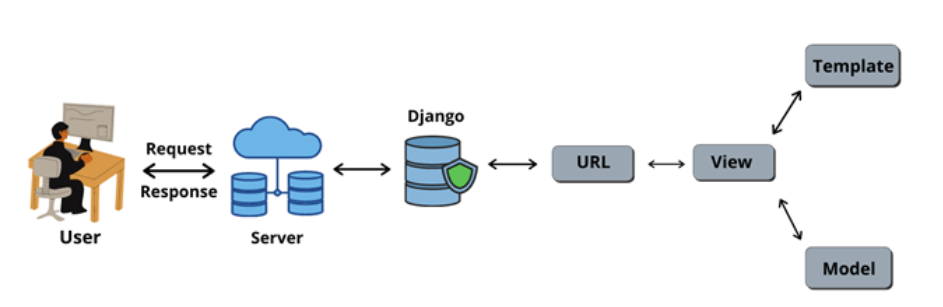
\includegraphics[width=0.5\textwidth]{graphics/django_architecture.png}
	\caption{Γενική αρχιτεκτονική του \en{Django}}
\end{figure}

\begin{itemize}
    \item  \en{Modularity}
    Καθώς η εφαρμογή μεγαλώνει, ο κώδικας πρέπει να είναι καλά δομημένος σε φακέλους
    και αρχεία ανάλογα με το τι κάνει ο κώδικας. Στο παρελθόν, οι μεγάλες εφαρμογές
    υπέφεραν όταν η εφαρμογή μεγάλωνε, υπήρχαν προβλήματα επεκτασιμότητας καθώς ο
    αριθμός των αρχείων \en{javascript} και \en{CSS} αυξανόταν ραγδαία και υπήρχαν
    πολύς επαναλαμβανόμενος κώδικας μεταξύ των αρχείων. Με την παροχή μιας καθορισμένης δομής,
    ένα συγκεκριμένο κομμάτι κώδικα μπορεί να αναζητηθεί εύκολα. Αν πάρουμε ως παράδειγμα
    παράδειγμα το πλαίσιο \en{Django}, το \en{Django} δομεί τον κώδικα σε ένα
    πολύ συγκεκριμένο τρόπο. 
    Μέσα στο αρχείο models.py ορίζονται τα μοντέλα της βάσης δεδομένων. Αυτό συμβαίνει προκειμένου να μπορούν να γίνουν
    ερωτήματα στη βάση δεδομένων που δεν σχετίζονται με τη συγκεκριμένη βάση δεδομένων που χρησιμοποιείται στο
    έργο. Μέσα στο αρχείο \en{views.py} γίνεται η λογική για την ανάκτηση και την επεξεργασία των δεδομένων όταν
    το ζητάει ο χρήστης. Μέσα στο αρχείο \en{urls.py} υλοποιείται η δρομολόγηση της
    εφαρμογής . Μέσα στο φάκελο \en{templates} υπάρχουν όλα τα \en{.html}
    αρχεία στα οποία το αρχείο \en{views.py} στέλνει τα δεδομένα που λαμβάνει για να τα απεικονίσει, κ.λπ.
    \item Ταχύτερη ανάπτυξη
    Τα πλαίσια παρέχουν έτοιμες λειτουργίες, καλώντας απλώς τις ήδη ενσωματωμένες συναρτήσεις/μεθόδους. Διαβάζοντας απλώς την τεκμηρίωση του πλαισίου και μαθαίνοντας πώς να τις χρησιμοποιεί, ο προγραμματιστής μπορεί να
    να ενσωματώσει λειτουργικότητες που διαφορετικά θα ήταν δύσκολο να υλοποιήσει
    και επίσης πολύ χρονοβόρες. Παραδείγματα περιλαμβάνουν λειτουργίες ελέγχου ταυτότητας, λειτουργίες διαχείρισης συνεδριών, λειτουργίες λειτουργίας βάσεων δεδομένων,
    λειτουργίες επικύρωσης φορμών και λειτουργίες για την παροχή ασφάλειας έναντι κακόβουλων επιτιθέμενων.
    \item Επέκταση κώδικα
    Τα περισσότερα \en{frameworks} επιτρέπουν την επέκταση κάποιου κομματιού κώδικα που θα χρησιμοποιηθεί
    σε πολλά άλλα αρχεία. Αυτό εξασφαλίζει ότι δεν υπάρχει επαναλαμβανόμενος κώδικας και
    οποιαδήποτε αλλαγή σε αυτόν τον κώδικα μεταφράζεται σε όλες τις περιπτώσεις που χρησιμοποιούν αυτόν τον κώδικα.
    \item Ευκολότερη αναγνωσιμότητα του κώδικα
    Δεδομένου ότι ο κώδικας χρησιμοποιεί καλά καθορισμένες τυποποιημένες συναρτήσεις και μια συγκεκριμένη δομή, είναι ευκολότερο να τον καταλάβει κάποιος που είναι νέος στο
    κώδικα αλλά γνωρίζει πώς λειτουργεί το πλαίσιο
\end{itemize}

\section{\en{CI/CD} \en{pipeline}}
Μόλις η εφαρμογή ιστού συνδεθεί με το απομακρυσμένο αποθετήριο, η τελευταία τάση στο
στον κόσμο του \en{DevOps} είναι η υλοποίηση ενός αγωγού \en{CI/CD}, ο οποίος ουσιαστικά
είναι μια αυτοματοποιημένη διαδικασία που ενεργοποιείται όταν νέος κώδικας δημοσιεύεται στο
απομακρυσμένο αποθετήριο. Αυτή η διαδικασία ξεκινάει τη δημιουργία κώδικα, εκτελεί κάποιες δοκιμές και
τέλος, αν όλα είναι εντάξει, αναπτύσσει αυτόματα τον κώδικα στην παραγωγή
περιβάλλον. Με αυτόν τον τρόπο, οι προγραμματιστές μπορούν να διασφαλίσουν ότι τίποτα δεν θα χαλάσει
στην παραγωγή και οι νέες λειτουργικότητες εξυπηρετούνται το συντομότερο δυνατό στους
πελάτη. Στην περίπτωσής μας τόσο η διπλωματική εργασία(\en{latex}) όσο και η εφαρμογή υλοποιήθηκαν με αυτή τη λογική.


\section{Τι είναι ο \en{kubernetes} }
Ο κυβερνήτης είναι ο διαχειριστής των με απλά λόγια ο διαχειριστής των \en{containers}. Είναι μια 
πλατφόρμα ανοικτού κώδικα για τη διαχείριση φορτίων εργασίας και υπηρεσιών που περιέχουν \en{containers}
, η οποία διευκολύνει τόσο τη δηλωτική διαμόρφωση όσο και την αυτοματοποίηση. 
Διαθέτει ένα μεγάλο, ταχέως αναπτυσσόμενο οικοσύστημα. Οι υπηρεσίες, η υποστήριξη και τα εργαλεία του \en{Kubernetes} είναι ευρέως διαθέσιμα.

\section{Τι είναι το \en{Docker} }
Το \en{Docker} είναι μια πλατφόρμα που επιτρέπει τη δημιουργία, τη διανομή και την εκτέλεση εφαρμογών μέσα σε ελαφριά, απομονωμένα "κοντέινερ" (\en{containers}). 
Τα κοντέινερ περιλαμβάνουν ό,τι χρειάζεται μια εφαρμογή για να τρέξει, όπως κώδικα, βιβλιοθήκες και εξαρτήσεις, διασφαλίζοντας ότι θα λειτουργεί ομοιόμορφα 
ανεξάρτητα από το περιβάλλον στο οποίο εκτελείται. Με αυτόν τον τρόπο διευκολύνει τη διαχείριση και τη μεταφορά εφαρμογών από τον έναν υπολογιστή ή διακομιστή 
στον άλλον.

\section{Τι είναι το \en{Git} }
Το \en{Git} είναι ένα σύγχρονο σύστημα ελέγχου εκδόσεων (γνωστό και ως σύστημα διαχείρισης αναθεωρήσεων ή πηγαίου κώδικα), 
σχεδιασμένο με έμφαση στην ταχύτητα, την ακεραιότητα των δεδομένων και την υποστήριξη κατανεμημένων, μη γραμμικών ροών εργασίας. 
Στην παρούσα διπλωματική εργασία, θα αξιοποιήσουμε το \en{Git} για να διασφαλίσουμε την ορθή διαχείριση των εκδόσεων του λογισμικού, 
τόσο κατά τη διάρκεια της ανάπτυξης όσο και για την πιθανή μελλοντική χρήση και εξέλιξη της δουλειάς μας. Το \en{GIT} συνεπώς είναι απαραίτητο σε κάθε σοβαρό 
έργο ανάπτυξης, και αυτό δεν αποτελεί εξαίρεση. Παρέχει γρήγορη ανάπτυξη κώδικα, έκδοση και επιτρέπει διακλαδώσεις. Έχοντας το εγκατεστημένο στον 
τοπικό υπολογιστή ανάπτυξης και στο περιβάλλον παραγωγής επιτρέπει την εύκολη και γρήγορη ανάπτυξη στο περιβάλλον παραγωγής.
τον ήδη δοκιμασμένο κώδικα στο τοπικό περιβάλλον ανάπτυξης. Η έκδοση παρέχει τη δυνατότητα επαναφοράς σε προηγούμενες εκδόσεις κώδικα σε
περίπτωση που κάποιο άγνωστο σφάλμα εμφανιστεί σε μια νεότερη έκδοση. 



%\begin{equation}
%	y = \alpha x + \beta
%\end{equation}

%Αντίθετα με αυτό που θεωρεί η πλειοψηφία, το \en{Lorem Ipsum} δεν είναι απλά ένα τυχαίο κείμενο. Οι ρίζες του βρίσκονται σε ένα κείμενο Λατινικής λογοτεχνίας του 45 π.Χ., φτάνοντας την ηλικία του πάνω από 2000 έτη.


%\begin{figure}[htb]
%	\centering
%	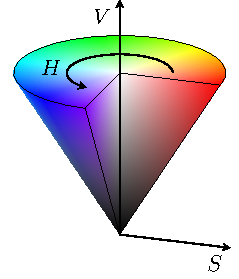
\includegraphics{tikz/hsv_cone/hsv_cone.pdf}
%	\caption{Ο χρωματικός χώρος \en{HSV}.}
%\end{figure}
